\documentclass[tikz,border=10pt]{standalone}
% Shared preamble for the CenterTask panel files (panel_a/b/c.tex).
% Edit colours and node styles here, once.
\usepackage{amsmath}
\usetikzlibrary{arrows.meta,positioning,calc}

% category colours as in ColorCategoryMap.m: 1=Short/Orange, 2=Mid/Green, 3=Long/Blue
\definecolor{catShort}{RGB}{243,178,132}
\definecolor{catMid}{RGB}{158,209,172}
\definecolor{catLong}{RGB}{157,188,234}

\tikzset{ctpanel/.style={
  font=\sffamily,
  band/.style={rounded corners=6pt, fill=black!7, draw=none, inner sep=8pt, minimum height=1.15cm},
  unit/.style={circle, fill=catMid!60, draw=none, minimum size=0.95cm, inner sep=0pt},
  flow/.style={-{Latex[length=2.2mm]}, line width=0.8pt},
  rowlab/.style={anchor=east, font=\sffamily\large},
  now/.style={fill=catShort!55, rounded corners=3pt, inner sep=3pt},
  stage/.style={rounded corners=6pt, fill=black!8, draw=none, inner sep=8pt, minimum height=1.2cm, align=center},
  target/.style={circle, minimum size=0.9cm, inner sep=0pt, draw=none, font=\sffamily\scriptsize, text=black!75},
  axis/.style={line width=0.6pt},
}}

\usepackage{amssymb}

% ---------------------------------------------------------------------
%  How each candidate model operationalises the same trial-level problem
%  (predict P(a_t) from the trial history and the current bar), in the
%  Ji-An framing: every model is a dynamical system with d state variables.
%  Columns: model-free RL, model-based RL, Bayesian observer, tiny RNN.
%  Rows: identical inputs; what the state IS; how it is UPDATED; how the
%  choice is READ OUT; what is fixed by the modeller vs fitted to data.
% ---------------------------------------------------------------------

\begin{document}
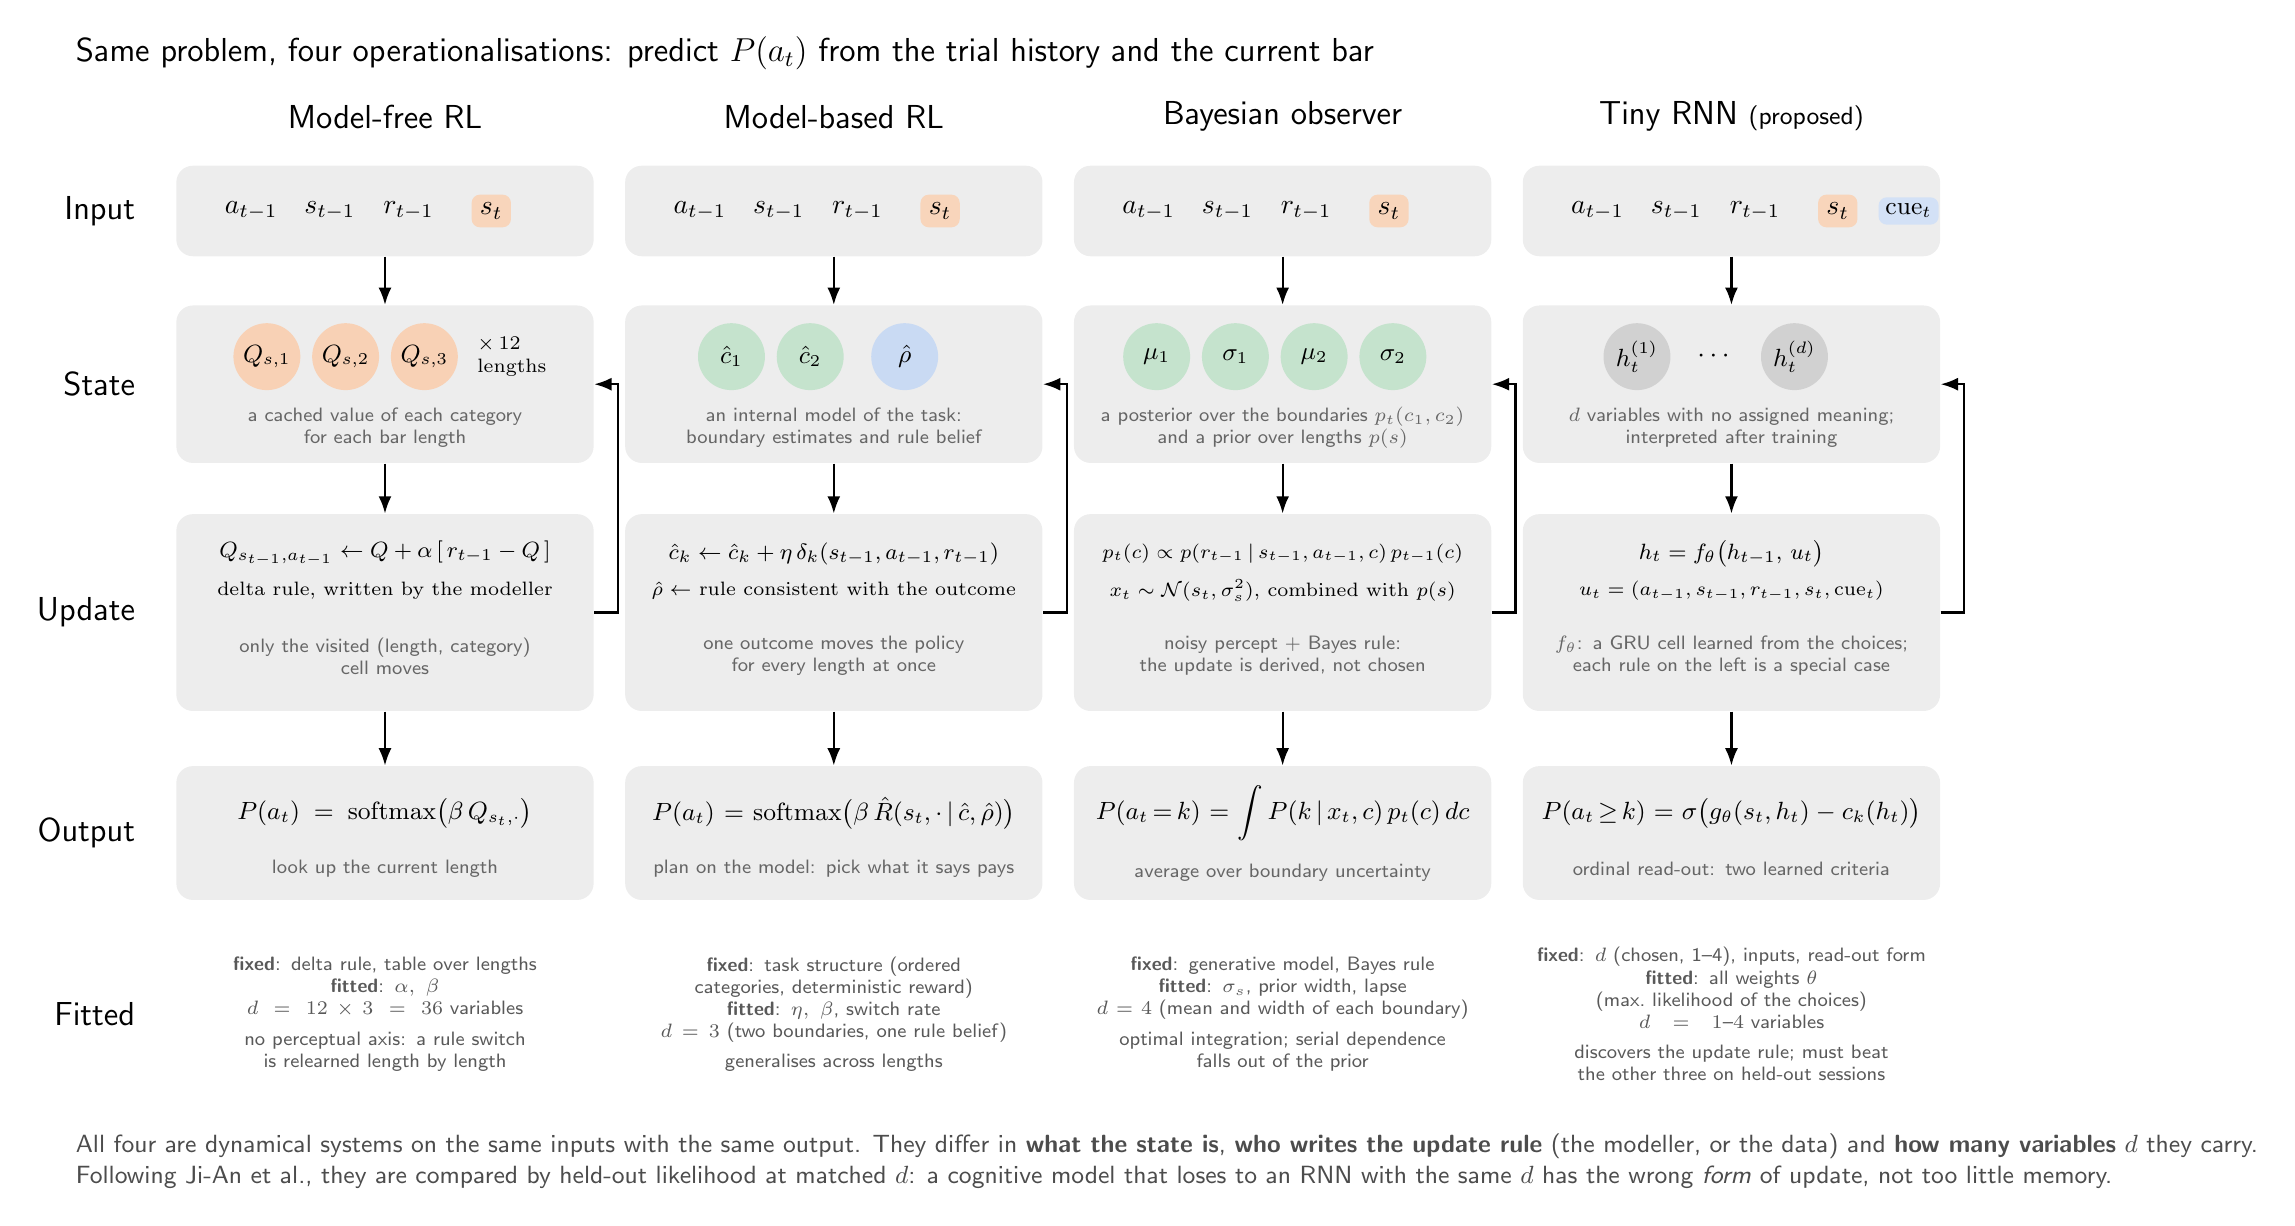
\begin{tikzpicture}[ctpanel,
  note/.style={text width=4.9cm, align=center, font=\sffamily\scriptsize, text=black!60},
  eq/.style={text width=5.0cm, align=center, font=\small},
  equ/.style={align=center, font=\footnotesize},
  eqs/.style={align=center, font=\scriptsize},
  fixed/.style={text width=5.0cm, align=center, font=\sffamily\scriptsize, text=black!65},
  hdr/.style={font=\sffamily\large, align=center, text width=5.2cm},
  state/.style={circle, fill=catMid!60, draw=none, minimum size=0.85cm, inner sep=0pt, font=\small},
  stateB/.style={circle, fill=catLong!55, draw=none, minimum size=0.85cm, inner sep=0pt, font=\small},
  stateQ/.style={circle, fill=catShort!60, draw=none, minimum size=0.85cm, inner sep=0pt, font=\small},
  stateH/.style={circle, fill=black!18, draw=none, minimum size=0.85cm, inner sep=0pt, font=\small},
]

% column centres and band geometry
\def\cw{5.3cm}
\def\xA{2.65}\def\xB{8.35}\def\xC{14.05}\def\xD{19.75}
\def\yIn{0}\def\yH{-2.2}\def\yU{-5.1}\def\yO{-7.9}\def\yF{-10.2}

\node[font=\sffamily\large, anchor=west] at (-1.4,2.0)
  {Same problem, four operationalisations: predict $P(a_t)$ from the trial history and the current bar};

% ---- row labels ----
\node[rowlab] at (-0.4,\yIn) {Input};
\node[rowlab] at (-0.4,\yH)  {State};
\node[rowlab] at (-0.4,\yU)  {Update};
\node[rowlab] at (-0.4,\yO)  {Output};
\node[rowlab] at (-0.4,\yF)  {Fitted};

% ---- column headers ----
\node[hdr] at (\xA,1.2) {Model-free RL};
\node[hdr] at (\xB,1.2) {Model-based RL};
\node[hdr] at (\xC,1.2) {Bayesian observer};
\node[hdr] at (\xD,1.2) {Tiny RNN {\small (proposed)}};

% ---- shared input band per column ----
\foreach \x in {\xA,\xB,\xC,\xD}{
  \node[band, minimum width=\cw] at (\x,\yIn) {};
  \node at (\x-1.7,\yIn) {$a_{t-1}$};
  \node at (\x-0.7,\yIn) {$s_{t-1}$};
  \node at (\x+0.3,\yIn) {$r_{t-1}$};
  \node[now] at (\x+1.35,\yIn) {$s_{t}$};
}
% the RNN also receives the rule cue as an input channel
\node[fill=catLong!45, rounded corners=3pt, inner sep=2.5pt, font=\small] at (\xD+2.25,\yIn) {$\mathrm{cue}_t$};

% =====================================================================
%  Column A: model-free RL
% =====================================================================
\node[band, minimum width=\cw, minimum height=2.0cm] (AH) at (\xA,\yH) {};
\node[stateQ] at (\xA-1.5,\yH+0.35) {$Q_{s,1}$};
\node[stateQ] at (\xA-0.5,\yH+0.35) {$Q_{s,2}$};
\node[stateQ] at (\xA+0.5,\yH+0.35) {$Q_{s,3}$};
\node[font=\scriptsize, anchor=west, align=left] at (\xA+1.05,\yH+0.35) {$\times\,12$\\ lengths};
\node[note] at (\xA,\yH-0.55) {a cached value of each category\\ for each bar length};

\node[band, minimum width=\cw, minimum height=2.5cm] (AU) at (\xA,\yU) {};
\node[equ] at (\xA,\yU+0.75) {$Q_{s_{t-1},a_{t-1}} \leftarrow Q + \alpha\,[\,r_{t-1}-Q\,]$};
\node[eqs] at (\xA,\yU+0.28) {delta rule, written by the modeller};
\node[note] at (\xA,\yU-0.55) {only the visited (length, category)\\ cell moves};

\node[band, minimum width=\cw, minimum height=1.7cm] (AO) at (\xA,\yO) {};
\node[eq] at (\xA,\yO+0.25) {$P(a_t)=\mathrm{softmax}\big(\beta\,Q_{s_t,\cdot}\big)$};
\node[note] at (\xA,\yO-0.45) {look up the current length};

\node[fixed] at (\xA,\yF)
  {\textbf{fixed}: delta rule, table over lengths\\
   \textbf{fitted}: $\alpha,\ \beta$\\
   $d = 12\times 3 = 36$ variables\\[3pt]
   no perceptual axis: a rule switch\\ is relearned length by length};

% =====================================================================
%  Column B: model-based RL
% =====================================================================
\node[band, minimum width=\cw, minimum height=2.0cm] (BH) at (\xB,\yH) {};
\node[state]  at (\xB-1.3,\yH+0.35) {$\hat{c}_1$};
\node[state]  at (\xB-0.3,\yH+0.35) {$\hat{c}_2$};
\node[stateB] at (\xB+0.9,\yH+0.35) {$\hat{\rho}$};
\node[note] at (\xB,\yH-0.55) {an internal model of the task:\\ boundary estimates and rule belief};

\node[band, minimum width=\cw, minimum height=2.5cm] (BU) at (\xB,\yU) {};
\node[equ] at (\xB,\yU+0.75) {$\hat{c}_k \leftarrow \hat{c}_k + \eta\,\delta_k(s_{t-1},a_{t-1},r_{t-1})$};
\node[eqs] at (\xB,\yU+0.28) {$\hat{\rho} \leftarrow$ rule consistent with the outcome};
\node[note] at (\xB,\yU-0.55) {one outcome moves the policy\\ for every length at once};

\node[band, minimum width=\cw, minimum height=1.7cm] (BO) at (\xB,\yO) {};
\node[eq] at (\xB,\yO+0.25) {$P(a_t)=\mathrm{softmax}\big(\beta\,\hat R(s_t,\cdot\,|\,\hat c,\hat\rho)\big)$};
\node[note] at (\xB,\yO-0.45) {plan on the model: pick what it says pays};

\node[fixed] at (\xB,\yF)
  {\textbf{fixed}: task structure (ordered\\ categories, deterministic reward)\\
   \textbf{fitted}: $\eta,\ \beta$, switch rate\\
   $d = 3$ (two boundaries, one rule belief)\\[3pt]
   generalises across lengths};

% =====================================================================
%  Column C: Bayesian observer
% =====================================================================
\node[band, minimum width=\cw, minimum height=2.0cm] (CH) at (\xC,\yH) {};
\node[state] at (\xC-1.6,\yH+0.35) {$\mu_1$};
\node[state] at (\xC-0.6,\yH+0.35) {$\sigma_1$};
\node[state] at (\xC+0.4,\yH+0.35) {$\mu_2$};
\node[state] at (\xC+1.4,\yH+0.35) {$\sigma_2$};
\node[note] at (\xC,\yH-0.55) {a posterior over the boundaries $p_t(c_1,c_2)$\\ and a prior over lengths $p(s)$};

\node[band, minimum width=\cw, minimum height=2.5cm] (CU) at (\xC,\yU) {};
\node[equ, font=\scriptsize] at (\xC,\yU+0.75) {$p_t(c)\propto p(r_{t-1}\,|\,s_{t-1},a_{t-1},c)\,p_{t-1}(c)$};
\node[eqs] at (\xC,\yU+0.28) {$x_t\sim\mathcal N(s_t,\sigma_s^2)$, combined with $p(s)$};
\node[note] at (\xC,\yU-0.55) {noisy percept + Bayes rule:\\ the update is derived, not chosen};

\node[band, minimum width=\cw, minimum height=1.7cm] (CO) at (\xC,\yO) {};
\node[eq] at (\xC,\yO+0.25) {$P(a_t\!=\!k)=\displaystyle\int P(k\,|\,x_t,c)\,p_t(c)\,dc$};
\node[note] at (\xC,\yO-0.5) {average over boundary uncertainty};

\node[fixed] at (\xC,\yF)
  {\textbf{fixed}: generative model, Bayes rule\\
   \textbf{fitted}: $\sigma_s$, prior width, lapse\\
   $d = 4$ (mean and width of each boundary)\\[3pt]
   optimal integration; serial dependence\\ falls out of the prior};

% =====================================================================
%  Column D: tiny RNN
% =====================================================================
\node[band, minimum width=\cw, minimum height=2.0cm] (DH) at (\xD,\yH) {};
\node[stateH] at (\xD-1.2,\yH+0.35) {$h^{(1)}_t$};
\node at (\xD-0.2,\yH+0.35) {$\cdots$};
\node[stateH] at (\xD+0.8,\yH+0.35) {$h^{(d)}_t$};
\node[note] at (\xD,\yH-0.55) {$d$ variables with no assigned meaning;\\ interpreted after training};

\node[band, minimum width=\cw, minimum height=2.5cm] (DU) at (\xD,\yU) {};
\node[equ] at (\xD,\yU+0.75) {$h_t = f_\theta\big(h_{t-1},\,u_t\big)$};
\node[eqs] at (\xD,\yU+0.28) {$u_t=(a_{t-1},s_{t-1},r_{t-1},s_t,\mathrm{cue}_t)$};
\node[note] at (\xD,\yU-0.55) {$f_\theta$: a GRU cell learned from the choices;\\ each rule on the left is a special case};

\node[band, minimum width=\cw, minimum height=1.7cm] (DO) at (\xD,\yO) {};
\node[eq] at (\xD,\yO+0.25) {$P(a_t\!\ge\!k)=\sigma\big(g_\theta(s_t,h_t)-c_k(h_t)\big)$};
\node[note] at (\xD,\yO-0.45) {ordinal read-out: two learned criteria};

\node[fixed] at (\xD,\yF)
  {\textbf{fixed}: $d$ (chosen, 1--4), inputs, read-out form\\
   \textbf{fitted}: all weights $\theta$\\ (max.\ likelihood of the choices)\\
   $d = 1$--$4$ variables\\[3pt]
   discovers the update rule; must beat\\ the other three on held-out sessions};

% ---- arrows: input -> state -> update -> output, plus recurrence ----
\foreach \x/\H/\U/\O in {\xA/AH/AU/AO, \xB/BH/BU/BO, \xC/CH/CU/CO, \xD/DH/DU/DO}{
  \draw[flow] (\x,\yIn-0.58) -- (\H.north);
  \draw[flow] (\H.south) -- (\U.north);
  \draw[flow] (\U.south) -- (\O.north);
  \draw[flow] (\U.east) -- ++(0.3,0) |- (\H.east);
}

% ---- footer ----
\node[align=left, anchor=north west, font=\sffamily\small, text=black!70] at (-1.4,-11.6) {%
  All four are dynamical systems on the same inputs with the same output. They differ in \textbf{what the state is},
  \textbf{who writes the update rule} (the modeller, or the data) and \textbf{how many variables} $d$ they carry.\\
  Following Ji-An et al., they are compared by held-out likelihood at matched $d$: a cognitive model that loses to an RNN
  with the same $d$ has the wrong \emph{form} of update, not too little memory.
};

\end{tikzpicture}
\end{document}
